\subsection{E-step versus sleep phase}
\label{sec:estep_sleep_compare}

In this subsection, we compare the posteriors obtained by optimizing the E-step objective~\eqref{eq:e_step} versus optimizing the sleep-phase objective~\eqref{eq:sleep_phase_summary}. 
We test on simulated data, so the wake-phase (M-step) is not needed. 

First, in 

% \begin{figure}[!ht]
%     \centering
%     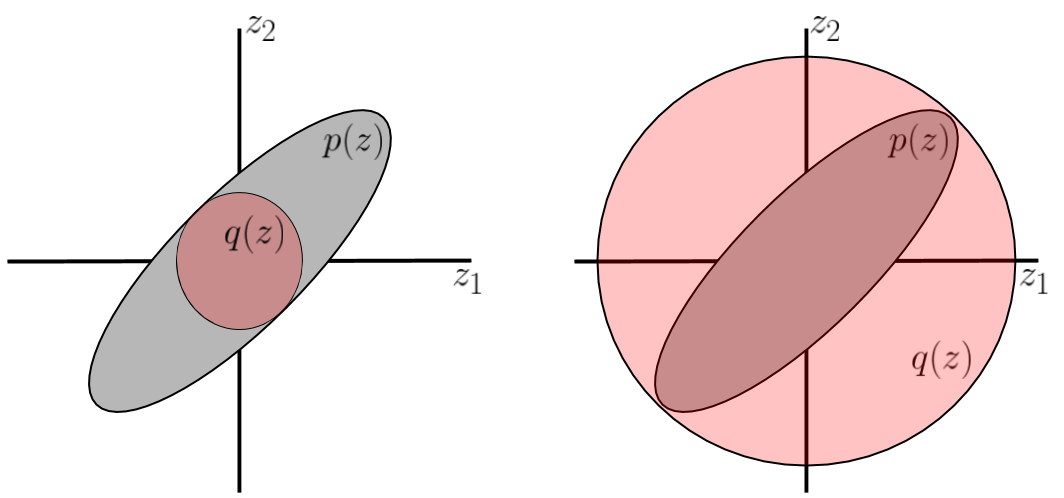
\includegraphics[width = 0.5\textwidth]{figures/kl_q_p_schematic.png}
%     \caption{A toy example where the target distribution $p$ is a bivariate Gaussian on 
%     $z = (z_1, z_2)$ with positively correlated components. 
%     $q$ is a mean-field variational approximation. Left, the optimal $q$ found 
%     optimizing $\KL(q\|p)$; right, the optimal $q$ found optimizing $\KL(p\|q)$. }
%     \jeff{Are the contour lines for $p$ and $q$ the same (e.g., the contour that contains 50\% of the mass)? If so, is it true that these contours touch at exactly two point (rather than 0 or 4)? We should be correct on this detail if we're going to the trouble of showing a plot, even if we're just trying to get intuition.}
%     \label{fig:kl_q_p_schematic}
% \end{figure}
